% !TeX spellcheck = it_IT
% !TeX root = ../../compl.tex
\section{Algoritmi Montecarlo e Las Vegas}

Un algoritmo probabilistico è un algoritmo che ha accesso a un oracolo che, a ogni chiamata, restituisce in tempo unitario un bit casuale, ovvero una variabile casuale $Y$ tale che $\Pr(Y = 1) = \Pr(Y = 0) = 1/2$. Inoltre, i bit restituiti in una sequenza di chiamate all'oracolo sono indipendenti.

Indicheremo con $Z \in \left\{0,1\right\}^\ast$ la stringa di bit casuali indipendenti che l'oracolo restituisce in una sequenza di chiamate. Indicheremo anche con $A(I, Z) \in \left\{0,1\right\}$ la variabile casuale che rappresenta l'output dell'algoritmo probabilistico $A$ per un problema di decisione $X = (\I, q)$ e avente come input l'istanza $I \in \I$ e i bit casuali $Z$ dell'oracolo. Similmente, indichiamo con $T_A (I, Z)$ la variabile casuale che rappresenta il tempo di esecuzione di $A$ con input $I \in \I$ e bit casuali $Z$ forniti dall'oracolo.

Esistono due principali tipi di algoritmi probabilistici.

\paragraph{Algoritmi Montecarlo.} Sono algoritmi $A$ tali che
\begin{itemize}
    \item Per ogni $I \in \I$, $T_A (I, Z)$ dipende solo da $I$, ovvero il tempo di esecuzione è deterministico

    \item Esiste $I \in \I$ per cui $\Pr \left(A(I, Z) \neq q(I)\right) > 0$, ovvero l'output non è sempre corretto
\end{itemize}

Gli algoritmi Montecarlo si dividono ulteriormente in:
\begin{itemize}
    \item Algoritmi con errore \textbf{one-sided}; un algoritmo ha errore one-sided quando è sempre corretto almeno su uno dei suoi due possibili output. Convenzionalmente, assumeremo che l'algoritmo sia sempre corretto per output 1. In altre parole, $A$ è Montecarlo one-sided quando, per ogni $I \in \I$, $\Pr \left(A(I, Z) = q(I) \mid A(I, Z) = 1\right) = 1$ e $\Pr \left(A(I, Z) = q(I) \mid A(I, Z) = 0\right) > 0$

    \item Algoritmi con errore \textbf{two-sided}. Possono sbagliare su entrambi i possibili output. Ovvero, $A$ è Montecarlo two-sided quando $\Pr\left(A(I,Z) = q(I)\right) > 1/2$ per ogni $I \in \I$
\end{itemize}

Una rappresentazione grafica della relazione fra $q(I)$ e $A(I,Z)$ per un algoritmo Montecarlo one-sided è la seguente
\begin{center}
    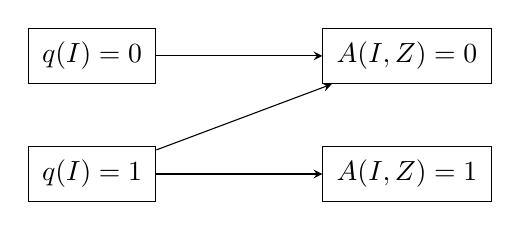
\begin{tikzpicture}[>=stealth]
    % Nodes
    \node[draw, inner sep=5pt] (q0) at (0, 1.5) {$q(I) = 0$};
    \node[draw, inner sep=5pt] (a0) at (4, 1.5) {$A(I, Z) = 0$};
    \node[draw, inner sep=5pt] (q1) at (0, 0)   {$q(I) = 1$};
    \node[draw, inner sep=5pt] (a1) at (4, 0)   {$A(I, Z) = 1$};
    % Arrows connecting the nodes
    \draw[->] (q0) -- (a0);
    \draw[->] (q1) -- (a1);
    \draw[->] (q1) -- (a0);
\end{tikzpicture}
\end{center}

Questo mostra come $A(I,Z) = 1$ può solo corrispondere a $q(I) = 1$, mentre $A(I,Z) = 0$ lascia incertezza sul valore di $q(I)$. Si noti anche che quando $q(I) = 0$ l'algoritmo è sempre corretto.

\paragraph{Algoritmi Las Vegas.} Sono algoritmi che producono sempre l'output corretto ma che hanno un tempo di esecuzione probabilistico (ovvero che dipende dai bit forniti dall'oracolo). Ovvero, un algoritmo $A$ è Las Vegas quando $\Pr\left(A(I,Z) = q(I)\right) = 1$ per ogni $I \in \I$ ma il tempo di calcolo di $A$ su una qualunque istanza $I \in \I$ è una variabile casuale $T_A (I,Z)$ tale che $\Ex\left[T_A (I,Z)\right] < \infty$.

\paragraph{Amplificazione.} Un algoritmo Montecarlo one-sided può essere facilmente trasformato in un algoritmo con probabilità di errore arbitrariamente piccola attraverso un meccanismo di amplificazione

Sia
$$ \Pr \left(A (I, Z) \neq q(I) \mid A(I, Z) = 0 \right) \leq 1 - p_n, \quad \forall I \in \I \text{ con } |I| = n $$
Se su una data istanza l'algoritmo produce 0 in output possiamo eseguirlo nuovamente per amplificare la probabilità di avere l'output corretto. Se $k$ esecuzioni indipendenti producono sistematicamente la risposta 0, allora la probabilità che la risposta corretta sia 1 è al più $\left(1 - p_n\right)^k \leq e^{-p_n k}$. Perché questa probabilità sia al più un $\epsilon > 0$ piccolo a piacere è sufficiente scegliere $k \geq \frac{1}{p_n} \ln \frac{1}{\epsilon}$.

Un meccanismo di amplificazione simile ma leggermente più complesso esiste anche per gli algoritmi Montecarlo two-sided. Supponiamo che su istanze di taglia $n$ l'algoritmo fornisca la risposta errata con probabilità al più $\frac{1}{2} - p_n < \frac{1}{2}$. Per amplificare la probabilità di ottenere la risposta corretta possiamo ripetere l'esecuzione $k$ volte e utilizzare un voto di maggioranza sui $k$ output prodotti (supponiamo, per semplicità, che $k$ sia dispari).

Per analizzare il voto di maggioranza utilizzeremo il seguente lemma. \\

\begin{lemma}[Chernoff-Hoeffding]
    \label{lemma:c-h}
    Siano $Y_1, \dots, Y_k$ variabili casuali Bernoulliane (cioè con valori in $\left\{0,1\right\}$), indipendenti e tali che $\Pr(Y_t = 1) \leq \mu$ per $t = 1, \dots, k$. Allora, per ogni $\epsilon > 0$ fissato
    $$ \Pr \left(\frac{1}{k} \sum_{t=1}^{k} Y_t > \mu + \epsilon\right) \leq e^{-2 \epsilon^2 k} $$
\end{lemma}
\begin{proof}
    Omessa.
\end{proof}

In altre parole, date delle variabili Bernoulliane indipendenti, con limite $\mu$ per il valore atteso, la disuguaglianza stabilisce la probabilità che la media si discosti di una certa quantità ($\epsilon$) dal valore atteso $\mu$. Intuitivamente, rappresenta la probabilità di allontanarsi dal valore atteso all'aumentare del numero di "tentativi" (variabili).

Sia $p_E = \Pr \left(A(I,Z) \neq q(I)\right)$ la probabilità di errore dell'algoritmo su un'istanza $I$ del problema di decisione $(\I, q)$. Siano $X_1, \dots, X_k \in \left\{0,1\right\}$ le variabili casuali indipendenti che denotano gli output prodotti dalle $k$ esecuzioni dell'algoritmo. Sia $M_k \in \left\{0,1\right\}$ la variabile casuale che denota il voto di maggioranza su $X_1, \dots, X_k$ (ovvero $M_k = 1$ se e solo se $\sum_{t=1}^k X_t > \frac{k}{2}$).

Allora
$$ M_k = q(I) \Longleftrightarrow \sum_{t=1}^k Y_t < \frac{k}{2} $$
dove $Y_t = 1$ se e solo se $X_t \neq q(I)$, per $t = 1, \dots, k$ (ovvero, se il risultato della relativa esecuzione dell'algoritmo è sbagliato). In altre parole, il voto di maggioranza $M_k$ è corretto se e solo se l'algoritmo genera output errato in non più di $\left\lfloor\frac{k}{2}\right\rfloor$ delle $k$ esecuzioni.

Ora, $Y_1, \dots, Y_k$ sono variabili casuali indipendenti (perché le esecuzioni dell'algoritmo sono indipendenti), identicamente distribuite, con valori in $\left\{0,1\right\}$ e tali che $\Pr (Y_t = 1) = p_E \leq \frac{1}{2} - p_n$ per ogni $t = 1, \dots, k$.

Applicando il lemma di Chernoff-Hoeffding (\ref{lemma:c-h}) otteniamo che la probabilità che il voto di maggioranza sia sbagliato è limitata da
\begin{align*}
    \Pr \left(\sum_{t=1}^k Y_t > \frac{k}{2}\right) & = \Pr \left(\frac{1}{k} \sum_{t=1}^k Y_t > \frac{1}{2} \right) \\
    & = \Pr \left(\frac{1}{k} \sum_{t=1}^k Y_t > \left(\frac{1}{2} - p_n\right) + p_n \right)  \\
    & \leq \Pr \left(\frac{1}{k} \sum_{t=1}^k Y_t > p_E + p_n \right)  \\
    & \leq e^{-2p_n^2 k}
\end{align*}

Perché la probabilità $e^{-2p_n^2k}$ sia al più un $\epsilon > 0$ piccolo a piacere è sufficiente scegliere
$$k \geq \frac{1}{2p^2_n} \ln \frac{1}{\epsilon}$$

Si noti che nel caso one-sided possiamo usare l'amplificazione per ridurre qualsiasi probabilità di errore strettamente minore di 1, mentre nel caso two-sided la stessa cosa vale per qualsiasi probabilità strettamente minore di $\frac{1}{2}$.

\paragraph{Da Las Vegas a Montecarlo one-sided.} Un algoritmo Las Vegas per un problema di decisione può essere trasformato in un algoritmo Montecarlo one-sided. Per fare ciò utilizziamo la disuguaglianza di Markov. \\

\begin{lemma}[Markov]
    \label{lemma:markov}
    Sia $Z$ una variabile casuale non negativa tale che $\Ex [Z] < \infty$. Allora per ogni $c > 0$
    $$ \Pr (Z > c) \leq \frac{\Ex [Z]}{c} $$
\end{lemma}
\begin{proof}
    Sia $\A$ l'insieme di numeri non negativi tali che $Z \in \A$. Allora
    \begin{align*}
        \Ex[Z] & = \sum_{a \in \A} a \Pr (Z = a) = \overbrace{\sum_{a \in \A: a \leq c} a \Pr(Z = a)}^{\geq 0} + \sum_{a \in \A: a > c} a \Pr (Z = a) \\
        & \geq c \sum_{a \in \A: a > c} \Pr (Z = a) \\
        & = c \Pr (Z = c)
    \end{align*}
    $$ \Ex [Z] \geq c \Pr (Z > c) \implies \Pr (Z > c) \leq \frac{\Ex[Z]}{c} $$
    concludendo la dimostrazione.
\end{proof}

Sia $A$ un algoritmo Las Vegas per un problema di decisione $(\I, q)$. Sia $f: \N \rightarrow \R$ la funzione tale che
$$ f(n) = \max \left\{\Ex \left[T_A (I,Z)\right] \mid I \in \I, \ |I| = n\right\}$$
In altre parole, la funzione rappresenta il massimo del valore atteso per il tempo di esecuzione dell'algoritmo $A$ per istanze di dimensione $n$.

Dato che $A$ è Las Vegas, $f(n) < \infty$ per ogni $n \in \N$. Possiamo quindi trovare una funzione $t: \N \rightarrow \N$ tale che
$$ t(n) \geq \frac{3}{2} f(n), \quad n \in \N $$

Posso quindi costruire un algoritmo $A'$ che simula $A$ sull'istanza $I$ arrestando la simulazione dopo $t(n)$ passi. Se $A$ non ha terminato, allora $A'$ produce 0 in output. Dato che $A$ è Las Vegas, $A'$ sbaglia solo quando $A$ non termina entro $t(n)$ passi. Per la disuguaglianza di Markov, la probabilità che ciò accada è al più
$$ \Pr \left(T_A (I, Z) > t(n)\right) \leq \frac{\Ex \left[T_A (I,Z)\right]}{t(n)} \leq \frac{f(n)}{t(n)} \leq \frac{2}{3} $$

Inoltre, dato che quando $A$ non termina l'output di $A'$ è 0, $A'$ è one-sided dato che l'output 1 è sempre corretto. Quindi $A'$ è un algoritmo Montecarlo one-sided con probabilità di errore al più $2/3$. Infine, si noti che il tempo di esecuzione di $A'$ soddisfa $T_{A'} (I) \leq t(|I|) = \O \left(f(|I|)\right)$.

\vfill

Riassumendo: un algoritmo Las Vegas può diventare Montecarlo one-sided con i seguenti passi
\begin{itemize}
    \item Trova una funzione $t(n)$ che maggiora la funzione $f(n)$, la quale rappresenta il tempo di esecuzione atteso per input di taglia $n$, ovvero $t(n) = m \cdot f(n)$

    \item L'algoritmo Montecarlo usa l'algoritmo Las Vegas, bloccando quest'ultimo se non termina entro $t(n)$ passi; restituisce sempre il risultato dell'algoritmo Las Vegas, oppure 0 se questo non termina

    \item La probabilità di errore è solo nel caso in cui esca 0; per la disuguaglianza di Markov, la probabilità che ciò accada è $\leq \frac{1}{m}$; quando esce 1, l'algoritmo è sempre corretto (quindi one-sided)
\end{itemize}

% end of probAlgo.pdf